\documentclass[twoside]{article}
\usepackage[]{dylan} % put copy for copyright, serif for serif font, utopia for utopia font, mathpazo for mathpazo font and hide to get rid of hints and small solutions, new for another style of theorems
 
\renewcommand{\abstractname}{\large\sffamily\bfseries\color{DylanBlue}Summary}
 
\title{Example File with dylan.sty}
\author{Dylan Yu}
\date{\today}
\runningheads{\textbf{Dylan Yu} (\today)}{Example File with dylan.sty}
 
\begin{document}
\maketitle

\begin{abstract}
Summarize what you are going to teach here. For example, today's topic is how to use \verb|dylan.sty|. Yay! I am writing more things to fill up the summary so you can see what it looks like.
\end{abstract}

\tableofcontents
\newpage

\section{Test}
\subsection{Testing}
\subsubsection{Tested}
\begin{defn}[Definition]
The word \vocab{definition} refers to the meaning of something.
\end{defn}
\begin{theorem}
Theorems, lemmas, corollaries, postulates, and propositions are all defined together. 
\end{theorem}
\begin{lemma}[Title of Lemma]
You can title all of these as well.
\end{lemma}
\begin{corollary}

\end{corollary}
\begin{postulate}

\end{postulate}
\begin{prop}

\end{prop}
\begin{proof}
We will use the following lemma:
\begin{lemma*}
This lemma is not numbered. Some unnumbered theorem styles are undefined, so create your own if necessary.
\end{lemma*}
\end{proof}
\begin{example}
Let $\alpha,\beta,\gamma$ be real numbers such that 
$$0\le \alpha,\beta,\gamma \le \frac{\pi}{2} \text{ and } \sin\alpha+\sin\beta+\sin\gamma=1.$$
Show that
$$\tan^2\alpha+\tan^2\beta+\tan^2\gamma\ge \frac{3}{8}.$$
\end{example}
\begin{soln}
Note that the domain of $\alpha,\beta,\gamma$ allows $\sin x,\cos x,\tan x$ to be nonnegative for all $x=\{\alpha,\beta,\gamma\}$. Applying Cauchy-Schwarz, we get
$$(\cos^2\alpha+\cos^2\beta+\cos^2\gamma)(\tan^2\alpha+\tan^2\beta+\tan^2\gamma)\ge (\cos\alpha\tan\alpha+\cos\beta\tan\beta+\cos\gamma+\tan\gamma)^2$$
$$\ge (\sin\alpha+\sin\beta+\sin\gamma)^2 = 1.$$
Furthermore, we know that by AM-GM,
$$\sqrt{\frac{\sin^2\alpha+\sin^2\beta+\sin^2\gamma}{3}} \ge \frac{\sin\alpha+\sin\beta+\sin\gamma}{3} = \frac{1}{3},$$
so $\sin^2\alpha+\sin^2\beta+\sin^2\gamma\ge \frac{1}{3}$. This implies that
$$3-(\sin^2\alpha+\sin^2\beta+\sin^2\gamma)\le 3-\frac{1}{3}=\frac{8}{3},$$
$$(1-\sin^2\alpha)+(1-\sin^2\beta)+(1-\sin^2\gamma)\le \frac{8}{3},$$
$$\cos^2\alpha+\cos^2\beta+\cos^2\gamma \le \frac{8}{3}.$$
Taking into account
$$(\cos^2\alpha+\cos^2\beta+\cos^2\gamma)(\tan^2\alpha+\tan^2\beta+\tan^2\gamma)\ge 1,$$
we get that
$$\frac{8}{3} (\tan^2\alpha+\tan^2\beta+\tan^2\gamma) \ge (\cos^2\alpha+\cos^2\beta+\cos^2\gamma)(\tan^2\alpha+\tan^2\beta+\tan^2\gamma)\ge 1,$$
so $\tan^2\alpha+\tan^2\beta+\tan^2\gamma\ge \frac{3}{8}$ as desired.
\end{soln}
\begin{problem}

\end{problem}
\begin{walk}
Explains the problem through steps:
\begin{enumerate}
    \item Read the problem.
    \item Read the problem again.
    \item Got it?
\end{enumerate}
\end{walk}

\begin{moral}
Use Dylan's .sty!
\end{moral}

\begin{fact}

\end{fact}

\begin{remark}

\end{remark}

\begin{basecase}

\end{basecase}

\begin{indstep}

\end{indstep}

\begin{case}

\end{case}

\begin{boxpar}[Paragraph Title]
Paragraphs are cool. This is a paragraph. It is very interesting. It even repeats! Replacing this with words you want will make the paragraph even better. Try it out! Paragraphs are cool. This is a paragraph. It is very interesting. It even repeats! Replacing this with words you want will make the paragraph even better. Try it out! Paragraphs are cool. This is a paragraph. It is very interesting. It even repeats! Replacing this with words you want will make the paragraph even better. Try it out!
\end{boxpar}

\begin{exercisebox}
\begin{exercise}
Consider $\triangle ABC$ with incenter $I.$ Prove that $\angle BIC=90^{\circ}+\frac{1}{2}\angle BAC.$
\end{exercise}
\begin{exercise}
If $1+1=3$, what is $2+2$?
\begin{hint}
\begin{addhint}
{This is a hint.}
\end{addhint}
\begin{addhint}
{You can add multiple hints.}
\end{addhint}
\end{hint}
\begin{sol}
\begin{addsol}
{You can also add solutions.}
\end{addsol}
\end{sol}
\end{exercise}
\begin{exercise}[Not a real problem]
How many beans are in my pocket?
\end{exercise}
\begin{exercise}
Exercise boxes can even go across pages!\footnote{This is a footnote.}
\end{exercise}
\end{exercisebox}

\begin{probbox}[red]
\item Problem
\item Problem
\item Problem
\item Problem
\item Problem
\item Problem
\item Problem
\item Problem
\item Problem
\item Problem
\item Problem
\item Problem
\end{probbox}

\begin{probbox}[MidnightBlue]
\item Problem
\item Problem
\item Problem
\item Problem
\item Problem
\item Problem
\item Problem
\item Problem
\item Problem
\item Problem
\item Problem
\item Problem
\end{probbox}

\begin{probbox}[ForestGreen]
\item Problem
\item Problem
\item Problem
\item Problem
\item Problem
\item Problem
\item Problem
\item Problem
\item Problem
\item Problem
\item Problem
\item Problem
\end{probbox}

\begin{probbox}
\item Problem
\item Problem
\item Problem
\item Problem
\item Problem
\item Problem
\item Problem
\item Problem
\item Problem
\item Problem
\item Problem
\item Problem
\end{probbox}

\begin{testbox}
\item Problem
\item Problem
\item Problem
\item Problem
\item Problem
\item Problem
\item Problem
\item Problem
\end{testbox}

\begin{testbox}[Test ]
\item Problem
\item Problem
\item Problem
\item Problem
\item Problem
\item Problem
\item Problem
\item Problem
\end{testbox}

\begin{figure}[H]
    \centering
    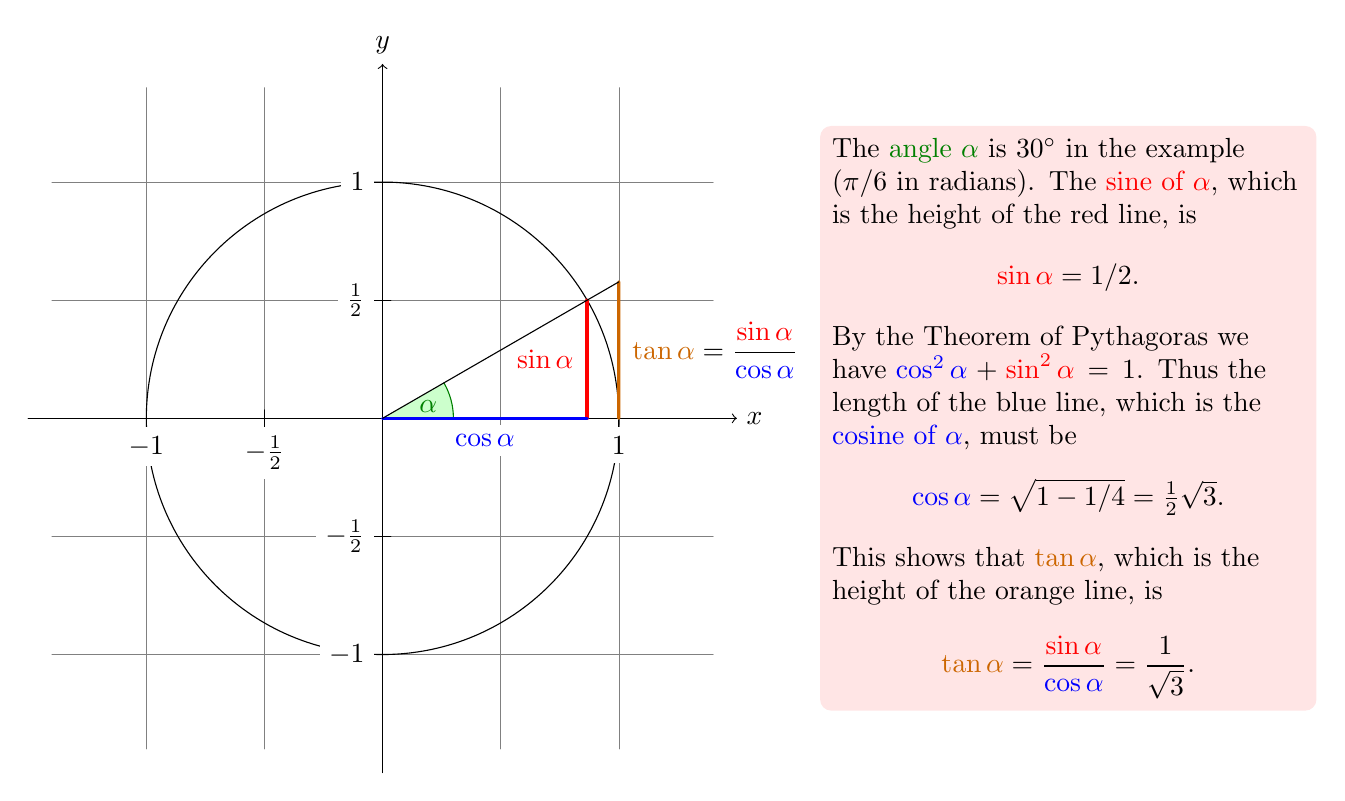
\begin{tikzpicture}[scale=3,cap=round]
      % Local definitions
      \def\costhirty{0.8660256}
    
      % Colors
      \colorlet{anglecolor}{green!50!black}
      \colorlet{sincolor}{red}
      \colorlet{tancolor}{orange!80!black}
      \colorlet{coscolor}{blue}
    
      % Styles
      \tikzstyle{axes}=[]
      \tikzstyle{important line}=[very thick]
      \tikzstyle{information text}=[rounded corners,fill=red!10,inner sep=1ex]
    
      % The graphic
      \draw[style=help lines,step=0.5cm] (-1.4,-1.4) grid (1.4,1.4);
    
      \draw (0,0) circle (1cm);
    
      \begin{scope}[style=axes]
        \draw[->] (-1.5,0) -- (1.5,0) node[right] {$x$};
        \draw[->] (0,-1.5) -- (0,1.5) node[above] {$y$};
    
        \foreach \x/\xtext in {-1, -.5/-\frac{1}{2}, 1}
          \draw[xshift=\x cm] (0pt,1pt) -- (0pt,-1pt) node[below,fill=white]
                {$\xtext$};
    
        \foreach \y/\ytext in {-1, -.5/-\frac{1}{2}, .5/\frac{1}{2}, 1}
          \draw[yshift=\y cm] (1pt,0pt) -- (-1pt,0pt) node[left,fill=white]
                {$\ytext$};
      \end{scope}
    
      \filldraw[fill=green!20,draw=anglecolor] (0,0) -- (3mm,0pt) arc(0:30:3mm);
      \draw (15:2mm) node[anglecolor] {$\alpha$};
    
      \draw[style=important line,sincolor]
        (30:1cm) -- node[left=1pt,fill=white] {$\sin \alpha$} +(0,-.5);
    
      \draw[style=important line,coscolor]
        (0,0) -- node[below=2pt,fill=white] {$\cos \alpha$} (\costhirty,0);
    
      \draw[style=important line,tancolor] (1,0) --
        node [right=1pt,fill=white]
        {
          $\displaystyle \tan \alpha \color{black}=
          \frac{{\color{sincolor}\sin \alpha}}{\color{coscolor}\cos \alpha}$
        } (intersection of 0,0--30:1cm and 1,0--1,1) coordinate (t);
    
      \draw (0,0) -- (t);
    
      \draw[xshift=1.85cm] node [right,text width=6cm,style=information text]
        {
          The {\color{anglecolor} angle $\alpha$} is $30^\circ$ in the
          example ($\pi/6$ in radians). The {\color{sincolor}sine of
            $\alpha$}, which is the height of the red line, is
          \[
          {\color{sincolor} \sin \alpha} = 1/2.
          \]
          By the Theorem of Pythagoras we have ${\color{coscolor}\cos^2 \alpha} +
          {\color{sincolor}\sin^2\alpha} =1$. Thus the length of the blue
          line, which is the {\color{coscolor}cosine of $\alpha$}, must be
          \[
          {\color{coscolor}\cos\alpha} = \sqrt{1 - 1/4} = \textstyle
          \frac{1}{2} \sqrt 3.
          \]%
          This shows that {\color{tancolor}$\tan \alpha$}, which is the
          height of the orange line, is
          \[
          {\color{tancolor}\tan\alpha} = \frac{{\color{sincolor}\sin
              \alpha}}{\color{coscolor}\cos \alpha} = \frac{1}{\sqrt 3}.
          \]%
        };
    \end{tikzpicture}
\end{figure}

\appendix % this makes the sections A,B,C,etc.
\pgfmathsetseed{2020} % or any other number: sets the random seed

% This is essentially the only way to reliably use loops, in the \makeatletter environment.
\makeatletter
\def\declarenumlist#1#2#3{%
\expandafter\edef\csname pgfmath@randomlist@#1\endcsname{#3}%
\count@\@ne
\loop
\expandafter\edef
\csname pgfmath@randomlist@#1@\the\count@\endcsname
  {\the\count@}
\ifnum\count@<#3\relax
\advance\count@\@ne
\repeat}

\declarenumlist{hintlist}{1}{\value{hintcounter}}

\def\prunelist#1{%
\expandafter\edef\csname pgfmath@randomlist@#1\endcsname
    {\the\numexpr\csname pgfmath@randomlist@#1\endcsname-1\relax}
\count@\pgfmath@randomtemp
\loop
\expandafter\let
\csname pgfmath@randomlist@#1@\the\count@\expandafter\endcsname
\csname pgfmath@randomlist@#1@\the\numexpr\count@+1\relax\endcsname
\ifnum\count@<\csname pgfmath@randomlist@#1\endcsname\relax
\advance\count@\@ne
\repeat}
\makeatother

\ifdylanhide

\else 
\section{Hints}
\hintprinter
\fi 

\pgfmathsetseed{2020} % or any other number: sets the random seed

%This is essentially the only way to reliably use loops, in the \makeatletter environment.
\makeatletter
\def\declarenumlist#1#2#3{%
\expandafter\edef\csname pgfmath@randomlist@#1\endcsname{#3}%
\count@\@ne
\loop
\expandafter\edef
\csname pgfmath@randomlist@#1@\the\count@\endcsname
  {\the\count@}
\ifnum\count@<#3\relax
\advance\count@\@ne
\repeat}

\declarenumlist{sollist}{1}{\value{solcounter}}

\def\prunelist#1{%
\expandafter\edef\csname pgfmath@randomlist@#1\endcsname
    {\the\numexpr\csname pgfmath@randomlist@#1\endcsname-1\relax}
\count@\pgfmath@randomtemp
\loop
\expandafter\let
\csname pgfmath@randomlist@#1@\the\count@\expandafter\endcsname
\csname pgfmath@randomlist@#1@\the\numexpr\count@+1\relax\endcsname
\ifnum\count@<\csname pgfmath@randomlist@#1\endcsname\relax
\advance\count@\@ne
\repeat}
\makeatother

\ifdylanhide

\else
\section{Solutions}
\solprinter
\fi


\end{document}
